In this section, we present additional experiments and use cases that showcase
\cockpit's utility. \Cref{cockpit::app:misscaled_data_exp_imagenet} shows that
\cockpit is able to scale to larger datasets by running the experiment with
incorrectly scaled data (see \Cref{cockpit::sec:misscaled_data_exp}) on
\imagenet instead of \cifarten. \Cref{cockpit::app:implicit_regularization_exp}
provides another concrete use case similar to \Cref{cockpit::fig:LINE}:
detecting regularization during training.

\subsection{Incorrectly Scaled Data for
  ImageNet}\label{cockpit::app:misscaled_data_exp_imagenet}

We repeat the experiment of \Cref{cockpit::sec:misscaled_data_exp} on the \imagenet
\citep{deng2009imagenet} dataset instead of \cifarten. We also use a larger neural
network model, switching from \threecthreed to \vgg \citep{simonyan2015deep}. This
demonstrates that \cockpit is able to scale to both larger models and datasets.
The input size of the images is almost fifty times larger ($224 \times 224$
instead of $32 \times 32$). The model size increased by roughly a factor of 150
(\vgg for \imagenet has roughly 138 million parameters, \threecthreed has less
than a million).

Similar to the example in the main text, the gradients are affected by the
scaling introduced via the input images, albeit less drastically (see
\Cref{cockpit::fig:data-pre-processing_imagenet}). Due to the gradient scaling,
default optimization hyperparameters might not work well anymore for the model
using the raw data.

\begin{figure*}[!t]
  \centering
  \begin{subfigure}[t]{0.46\linewidth}
    \begin{minipage}{.49\linewidth}
      \Cshadowbox{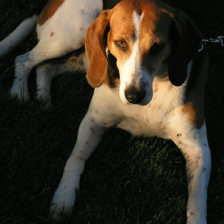
\includegraphics[width =
        .35\linewidth]{../repos/cockpit-paper/tex/fig/06_preprocessing/fig_samples/imagenetraw_vgg16_sample_00.png}}
      \Cshadowbox{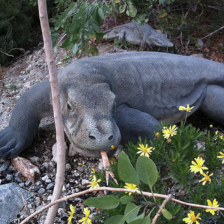
\includegraphics[width =
        .35\linewidth]{../repos/cockpit-paper/tex/fig/06_preprocessing/fig_samples/imagenetraw_vgg16_sample_01.png}}

      \Cshadowbox{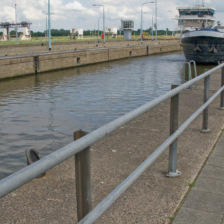
\includegraphics[width =
        .35\linewidth]{../repos/cockpit-paper/tex/fig/06_preprocessing/fig_samples/imagenetraw_vgg16_sample_02.png}}
      \Cshadowbox{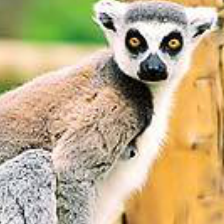
\includegraphics[width =
        .35\linewidth]{../repos/cockpit-paper/tex/fig/06_preprocessing/fig_samples/imagenetraw_vgg16_sample_03.png}}
    \end{minipage}
    \begin{minipage}{.49\linewidth}
      \pgfkeys{/pgfplots/preprocessingexperimentdefault/.style={
    width=1.15\linewidth,
    height=1.22\linewidth,
    every axis plot/.append style={line width = 1.5pt},
    tick pos = left,
    xmajorticks = true,
    ymajorticks = true,
    ylabel near ticks,
    xlabel near ticks,
    xtick align = inside,
    ytick align = inside,
    legend cell align = left,
    legend columns = 1,
    legend pos = south east,
    legend style = {
      fill opacity = 0.7,
      text opacity = 1,
      font = \footnotesize,
    },
    xticklabel style = {font = \footnotesize, inner xsep = 0ex},
    xlabel style = {font = \footnotesize},
    axis line style = {black},
    yticklabel style = {font = \footnotesize, inner ysep = -4ex},
    ylabel style = {font = \footnotesize},
    title style = {font = \footnotesize, inner ysep = -3ex},
    grid = major,
    grid style = {dashed}
  }
}
%%% Local Variables:
%%% mode: latex
%%% TeX-master: "../../../thesis"
%%% End:

      \centering
      % customize "zmystyle" as you wish
      \pgfkeys{/pgfplots/zmystyle/.style={preprocessingexperimentdefault,
          ylabel={Gradient Element}
        }}
      \vspace{1.4\baselineskip}
      \tikzexternalenable
      % This file was created with tikzplotlib v0.9.14.
\begin{tikzpicture}

\definecolor{color0}{rgb}{0.12156862745098,0.466666666666667,0.705882352941177}

\begin{axis}[
axis line style={white},
log basis x={10},
tick align=outside,
xmajorticks=false,
xmin=0.9, xmax=315917612.324796,
xmode=log,
xtick style={color=white!15!black},
ymajorticks=false,
ymin=-1.5, ymax=1.5,
zmystyle
]
\draw[draw=white,fill=color0,line width=0.04pt] (axis cs:0.9,-1.5) rectangle (axis cs:0.9,-1.42499995231628);
\draw[draw=white,fill=color0,line width=0.04pt] (axis cs:0.9,-1.42500007152557) rectangle (axis cs:0.9,-1.35000002384186);
\draw[draw=white,fill=color0,line width=0.04pt] (axis cs:0.9,-1.35000002384186) rectangle (axis cs:0.9,-1.27499997615814);
\draw[draw=white,fill=color0,line width=0.04pt] (axis cs:0.9,-1.27499997615814) rectangle (axis cs:0.9,-1.19999992847443);
\draw[draw=white,fill=color0,line width=0.04pt] (axis cs:0.9,-1.20000004768372) rectangle (axis cs:0.9,-1.125);
\draw[draw=white,fill=color0,line width=0.04pt] (axis cs:0.9,-1.125) rectangle (axis cs:0.9,-1.04999995231628);
\draw[draw=white,fill=color0,line width=0.04pt] (axis cs:0.9,-1.04999995231628) rectangle (axis cs:0.9,-0.974999904632568);
\draw[draw=white,fill=color0,line width=0.04pt] (axis cs:0.9,-0.975000023841858) rectangle (axis cs:0.9,-0.899999976158142);
\draw[draw=white,fill=color0,line width=0.04pt] (axis cs:0.9,-0.899999976158142) rectangle (axis cs:0.9,-0.824999928474426);
\draw[draw=white,fill=color0,line width=0.04pt] (axis cs:0.9,-0.825000047683716) rectangle (axis cs:0.9,-0.75);
\draw[draw=white,fill=color0,line width=0.04pt] (axis cs:0.9,-0.75) rectangle (axis cs:0.9,-0.674999952316284);
\draw[draw=white,fill=color0,line width=0.04pt] (axis cs:0.9,-0.674999952316284) rectangle (axis cs:0.9,-0.599999904632568);
\draw[draw=white,fill=color0,line width=0.04pt] (axis cs:0.9,-0.600000023841858) rectangle (axis cs:0.9,-0.524999976158142);
\draw[draw=white,fill=color0,line width=0.04pt] (axis cs:0.9,-0.524999976158142) rectangle (axis cs:0.9,-0.449999928474426);
\draw[draw=white,fill=color0,line width=0.04pt] (axis cs:0.9,-0.449999988079071) rectangle (axis cs:0.9,-0.374999940395355);
\draw[draw=white,fill=color0,line width=0.04pt] (axis cs:0.9,-0.374999970197678) rectangle (axis cs:0.9,-0.299999922513962);
\draw[draw=white,fill=color0,line width=0.04pt] (axis cs:0.9,-0.299999982118607) rectangle (axis cs:0.9,-0.224999934434891);
\draw[draw=white,fill=color0,line width=0.04pt] (axis cs:0.9,-0.224999964237213) rectangle (axis cs:3.9,-0.149999916553497);
\draw[draw=white,fill=color0,line width=0.04pt] (axis cs:0.9,-0.149999968707561) rectangle (axis cs:102.9,-0.0749999210238457);
\draw[draw=white,fill=color0,line width=0.04pt] (axis cs:0.9,-0.075000025331974) rectangle (axis cs:123780803.9,2.23517417907715e-08);
\draw[draw=white,fill=color0,line width=0.04pt] (axis cs:0.9,-8.19563865661621e-08) rectangle (axis cs:14580628.9,0.0749999657273293);
\draw[draw=white,fill=color0,line width=0.04pt] (axis cs:0.9,0.0749999210238457) rectangle (axis cs:98.9,0.149999968707561);
\draw[draw=white,fill=color0,line width=0.04pt] (axis cs:0.9,0.149999916553497) rectangle (axis cs:6.9,0.224999964237213);
\draw[draw=white,fill=color0,line width=0.04pt] (axis cs:0.9,0.224999934434891) rectangle (axis cs:0.9,0.299999982118607);
\draw[draw=white,fill=color0,line width=0.04pt] (axis cs:0.9,0.299999922513962) rectangle (axis cs:0.9,0.374999970197678);
\draw[draw=white,fill=color0,line width=0.04pt] (axis cs:0.9,0.374999940395355) rectangle (axis cs:0.9,0.449999988079071);
\draw[draw=white,fill=color0,line width=0.04pt] (axis cs:0.9,0.449999928474426) rectangle (axis cs:0.9,0.524999976158142);
\draw[draw=white,fill=color0,line width=0.04pt] (axis cs:0.9,0.524999976158142) rectangle (axis cs:0.9,0.600000023841858);
\draw[draw=white,fill=color0,line width=0.04pt] (axis cs:0.9,0.599999904632568) rectangle (axis cs:0.9,0.674999952316284);
\draw[draw=white,fill=color0,line width=0.04pt] (axis cs:0.9,0.674999952316284) rectangle (axis cs:0.9,0.75);
\draw[draw=white,fill=color0,line width=0.04pt] (axis cs:0.9,0.75) rectangle (axis cs:0.9,0.825000047683716);
\draw[draw=white,fill=color0,line width=0.04pt] (axis cs:0.9,0.824999928474426) rectangle (axis cs:0.9,0.899999976158142);
\draw[draw=white,fill=color0,line width=0.04pt] (axis cs:0.9,0.899999976158142) rectangle (axis cs:0.9,0.975000023841858);
\draw[draw=white,fill=color0,line width=0.04pt] (axis cs:0.9,0.974999904632568) rectangle (axis cs:1.9,1.04999995231628);
\draw[draw=white,fill=color0,line width=0.04pt] (axis cs:0.9,1.04999995231628) rectangle (axis cs:0.9,1.125);
\draw[draw=white,fill=color0,line width=0.04pt] (axis cs:0.9,1.125) rectangle (axis cs:0.9,1.20000004768372);
\draw[draw=white,fill=color0,line width=0.04pt] (axis cs:0.9,1.19999992847443) rectangle (axis cs:0.9,1.27499997615814);
\draw[draw=white,fill=color0,line width=0.04pt] (axis cs:0.9,1.27499997615814) rectangle (axis cs:0.9,1.35000002384186);
\draw[draw=white,fill=color0,line width=0.04pt] (axis cs:0.9,1.35000002384186) rectangle (axis cs:0.9,1.42500007152557);
\draw[draw=white,fill=color0,line width=0.04pt] (axis cs:0.9,1.42499995231628) rectangle (axis cs:0.9,1.5);
\end{axis}

\end{tikzpicture}

      \tikzexternaldisable
    \end{minipage}
    \vspace{-2ex}
    \caption{Normalized Data}
    \label{cockpit::fig:data-pre-processing_norm_imagenet}
  \end{subfigure}
  \hfill
  \begin{subfigure}[t]{0.46\linewidth}
    \begin{minipage}{.49\linewidth}
      \Cshadowbox{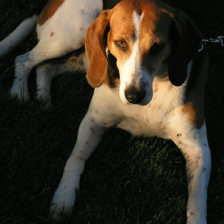
\includegraphics[width =
        .35\linewidth]{../repos/cockpit-paper/tex/fig/06_preprocessing/fig_samples/imagenetscale255_vgg16_sample_00.png}}
      \Cshadowbox{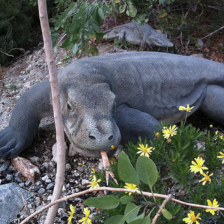
\includegraphics[width =
        .35\linewidth]{../repos/cockpit-paper/tex/fig/06_preprocessing/fig_samples/imagenetscale255_vgg16_sample_01.png}}

      \Cshadowbox{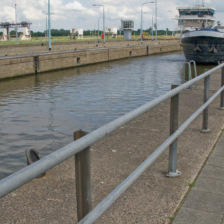
\includegraphics[width =
        .35\linewidth]{../repos/cockpit-paper/tex/fig/06_preprocessing/fig_samples/imagenetscale255_vgg16_sample_02.png}}
      \Cshadowbox{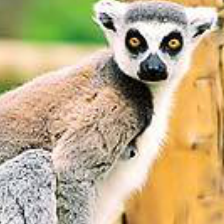
\includegraphics[width =
        .35\linewidth]{../repos/cockpit-paper/tex/fig/06_preprocessing/fig_samples/imagenetscale255_vgg16_sample_03.png}}
    \end{minipage}
    \begin{minipage}{.49\linewidth}
      \centering
      \pgfkeys{/pgfplots/preprocessingexperimentdefault/.style={
    width=1.15\linewidth,
    height=1.22\linewidth,
    every axis plot/.append style={line width = 1.5pt},
    tick pos = left,
    xmajorticks = true,
    ymajorticks = true,
    ylabel near ticks,
    xlabel near ticks,
    xtick align = inside,
    ytick align = inside,
    legend cell align = left,
    legend columns = 1,
    legend pos = south east,
    legend style = {
      fill opacity = 0.7,
      text opacity = 1,
      font = \footnotesize,
    },
    xticklabel style = {font = \footnotesize, inner xsep = 0ex},
    xlabel style = {font = \footnotesize},
    axis line style = {black},
    yticklabel style = {font = \footnotesize, inner ysep = -4ex},
    ylabel style = {font = \footnotesize},
    title style = {font = \footnotesize, inner ysep = -3ex},
    grid = major,
    grid style = {dashed}
  }
}
%%% Local Variables:
%%% mode: latex
%%% TeX-master: "../../../thesis"
%%% End:

      % customize "zmystyle" as you wish
      \pgfkeys{/pgfplots/zmystyle/.style={preprocessingexperimentdefault,
          ylabel={Gradient Element}
        }}
      \vspace{1.4\baselineskip}
      \tikzexternalenable
      % This file was created with tikzplotlib v0.9.14.
\begin{tikzpicture}

\definecolor{color0}{rgb}{1,0.498039215686275,0.0549019607843137}

\begin{axis}[
axis line style={white},
log basis x={10},
tick align=outside,
xmajorticks=false,
xmin=0.9, xmax=315354991.80789,
xmode=log,
xtick style={color=white!15!black},
ymajorticks=false,
ymin=-1.5, ymax=1.5,
zmystyle
]
\draw[draw=white,fill=color0,line width=0.04pt] (axis cs:0.9,-1.5) rectangle (axis cs:0.9,-1.42499995231628);
\draw[draw=white,fill=color0,line width=0.04pt] (axis cs:0.9,-1.42500007152557) rectangle (axis cs:0.9,-1.35000002384186);
\draw[draw=white,fill=color0,line width=0.04pt] (axis cs:0.9,-1.35000002384186) rectangle (axis cs:0.9,-1.27499997615814);
\draw[draw=white,fill=color0,line width=0.04pt] (axis cs:0.9,-1.27499997615814) rectangle (axis cs:0.9,-1.19999992847443);
\draw[draw=white,fill=color0,line width=0.04pt] (axis cs:0.9,-1.20000004768372) rectangle (axis cs:0.9,-1.125);
\draw[draw=white,fill=color0,line width=0.04pt] (axis cs:0.9,-1.125) rectangle (axis cs:0.9,-1.04999995231628);
\draw[draw=white,fill=color0,line width=0.04pt] (axis cs:0.9,-1.04999995231628) rectangle (axis cs:0.9,-0.974999904632568);
\draw[draw=white,fill=color0,line width=0.04pt] (axis cs:0.9,-0.975000023841858) rectangle (axis cs:0.9,-0.899999976158142);
\draw[draw=white,fill=color0,line width=0.04pt] (axis cs:0.9,-0.899999976158142) rectangle (axis cs:0.9,-0.824999928474426);
\draw[draw=white,fill=color0,line width=0.04pt] (axis cs:0.9,-0.825000047683716) rectangle (axis cs:0.9,-0.75);
\draw[draw=white,fill=color0,line width=0.04pt] (axis cs:0.9,-0.75) rectangle (axis cs:0.9,-0.674999952316284);
\draw[draw=white,fill=color0,line width=0.04pt] (axis cs:0.9,-0.674999952316284) rectangle (axis cs:0.9,-0.599999904632568);
\draw[draw=white,fill=color0,line width=0.04pt] (axis cs:0.9,-0.600000023841858) rectangle (axis cs:0.9,-0.524999976158142);
\draw[draw=white,fill=color0,line width=0.04pt] (axis cs:0.9,-0.524999976158142) rectangle (axis cs:0.9,-0.449999928474426);
\draw[draw=white,fill=color0,line width=0.04pt] (axis cs:0.9,-0.449999988079071) rectangle (axis cs:0.9,-0.374999940395355);
\draw[draw=white,fill=color0,line width=0.04pt] (axis cs:0.9,-0.374999970197678) rectangle (axis cs:0.9,-0.299999922513962);
\draw[draw=white,fill=color0,line width=0.04pt] (axis cs:0.9,-0.299999982118607) rectangle (axis cs:40.9,-0.224999934434891);
\draw[draw=white,fill=color0,line width=0.04pt] (axis cs:0.9,-0.224999964237213) rectangle (axis cs:872.9,-0.149999916553497);
\draw[draw=white,fill=color0,line width=0.04pt] (axis cs:0.9,-0.149999968707561) rectangle (axis cs:45198.9,-0.0749999210238457);
\draw[draw=white,fill=color0,line width=0.04pt] (axis cs:0.9,-0.075000025331974) rectangle (axis cs:123570849.9,2.23517417907715e-08);
\draw[draw=white,fill=color0,line width=0.04pt] (axis cs:0.9,-8.19563865661621e-08) rectangle (axis cs:14693460.9,0.0749999657273293);
\draw[draw=white,fill=color0,line width=0.04pt] (axis cs:0.9,0.0749999210238457) rectangle (axis cs:48872.9,0.149999968707561);
\draw[draw=white,fill=color0,line width=0.04pt] (axis cs:0.9,0.149999916553497) rectangle (axis cs:1580.9,0.224999964237213);
\draw[draw=white,fill=color0,line width=0.04pt] (axis cs:0.9,0.224999934434891) rectangle (axis cs:137.9,0.299999982118607);
\draw[draw=white,fill=color0,line width=0.04pt] (axis cs:0.9,0.299999922513962) rectangle (axis cs:91.9,0.374999970197678);
\draw[draw=white,fill=color0,line width=0.04pt] (axis cs:0.9,0.374999940395355) rectangle (axis cs:74.9,0.449999988079071);
\draw[draw=white,fill=color0,line width=0.04pt] (axis cs:0.9,0.449999928474426) rectangle (axis cs:73.9,0.524999976158142);
\draw[draw=white,fill=color0,line width=0.04pt] (axis cs:0.9,0.524999976158142) rectangle (axis cs:62.9,0.600000023841858);
\draw[draw=white,fill=color0,line width=0.04pt] (axis cs:0.9,0.599999904632568) rectangle (axis cs:44.9,0.674999952316284);
\draw[draw=white,fill=color0,line width=0.04pt] (axis cs:0.9,0.674999952316284) rectangle (axis cs:58.9,0.75);
\draw[draw=white,fill=color0,line width=0.04pt] (axis cs:0.9,0.75) rectangle (axis cs:54.9,0.825000047683716);
\draw[draw=white,fill=color0,line width=0.04pt] (axis cs:0.9,0.824999928474426) rectangle (axis cs:45.9,0.899999976158142);
\draw[draw=white,fill=color0,line width=0.04pt] (axis cs:0.9,0.899999976158142) rectangle (axis cs:27.9,0.975000023841858);
\draw[draw=white,fill=color0,line width=0.04pt] (axis cs:0.9,0.974999904632568) rectangle (axis cs:21.9,1.04999995231628);
\draw[draw=white,fill=color0,line width=0.04pt] (axis cs:0.9,1.04999995231628) rectangle (axis cs:23.9,1.125);
\draw[draw=white,fill=color0,line width=0.04pt] (axis cs:0.9,1.125) rectangle (axis cs:12.9,1.20000004768372);
\draw[draw=white,fill=color0,line width=0.04pt] (axis cs:0.9,1.19999992847443) rectangle (axis cs:11.9,1.27499997615814);
\draw[draw=white,fill=color0,line width=0.04pt] (axis cs:0.9,1.27499997615814) rectangle (axis cs:12.9,1.35000002384186);
\draw[draw=white,fill=color0,line width=0.04pt] (axis cs:0.9,1.35000002384186) rectangle (axis cs:6.9,1.42500007152557);
\draw[draw=white,fill=color0,line width=0.04pt] (axis cs:0.9,1.42499995231628) rectangle (axis cs:20.9,1.5);
\end{axis}

\end{tikzpicture}

      \tikzexternaldisable
    \end{minipage}
    \vspace{-2ex}
    \caption{Raw Data}
    \label{cockpit::fig:data-pre-processing_raw_imagenet}
  \end{subfigure}
  \caption{\textbf{Same inputs, different gradients on ImageNet.} This is
    structurally the same plot as \Cref{cockpit::fig:data-pre-processing}, but
    using \imagenet and \vgg.
    \subfigref{cockpit::fig:data-pre-processing_norm_imagenet} \emph{normalized}
    ($[0, 1]$) and \subfigref{cockpit::fig:data-pre-processing_raw_imagenet}
    \emph{raw} $([0, 255])$ images look identical in auto-scaled front-ends like
    \matplotlib's \robustInlinecode{imshow}. The gradient distribution on the \vgg model,
    however, is affected by this scaling.}
  \label{cockpit::fig:data-pre-processing_imagenet}
\end{figure*}

%%% Local Variables:
%%% mode: latex
%%% TeX-master: "../../../thesis"
%%% End:


%%% Local Variables:
%%% mode: latex
%%% TeX-master: "../thesis"
%%% End:
